	\subsection*{Report 5 + 6}
	When the sample size is small, the resolution of corresponding FFT is limited as demonstrated in the previous report. If the time domain signal is zero-padded, the longer time signal will yield an interpolated signal in the frequency domain. This effect is shown below in figure \ref{figure:2_3}, where the original signal and zero padded signal show the clear interpolation that occurs as a result of zero padding. The MATLAB script that was used can be found on page \pageref{matlab_2.3}.
	
	\begin{figure}[H] 
		\centering
		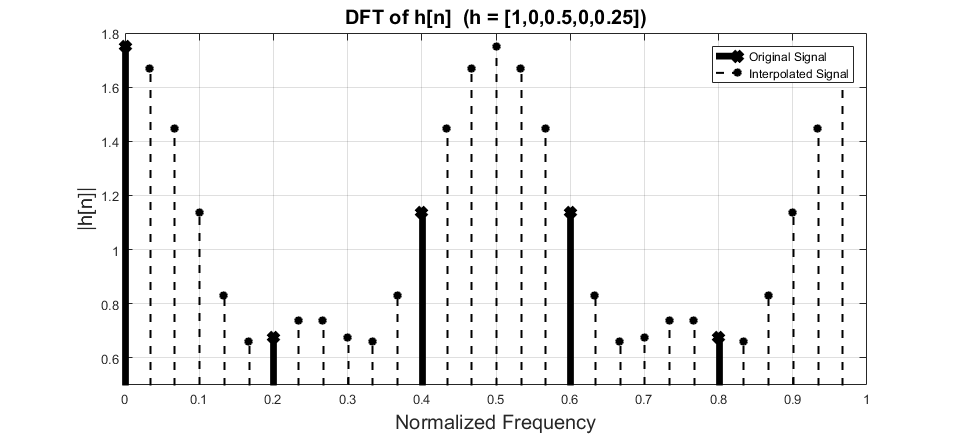
\includegraphics[width=\textwidth]{2.3.png}
		\caption{Interpolated sequence with DFT through zero padding}
		\label{figure:2_3}
	\end{figure}